\section{Stage VII: Measuring With Safepoints On}
\label{sec:reality}

\subsection{Two Compiler Configurations}
Whether the compiler inserts safepoint polls is a configure option fixed when
it is built. The compilers of Sections~\ref{sec:sr} to~\ref{sec:stage6} were
built with \code{--enable-flambda2} alone, which inserts no polls. The release
also passes \code{--enable-poll-insertion} (Listing~\ref{lst:config}); this
stage measures the passes in that configuration.

\begin{lstlisting}[language=plaintext,caption={Configure options of the compilers of Stages IV--VI (top) and of the opam OxCaml release (bottom).},label=lst:config,numbers=none]
# compilers of Stages IV-VI
--enable-flambda2                      -> POLL_INSERTION=false

# opam release recipe, oxcaml-compiler 5.4.0-ox7
--enable-middle-end=flambda2 --enable-runtime5 --enable-stack-checks
--enable-poll-insertion --enable-multidomain
\end{lstlisting}

\subsection{What the Passes Are Worth With Safepoints}
\label{tab:pollladder}
On the pull-request compiler with the release options, four builds (passes
off and on, each with and without polls) produce identical output. Without
polls the
passes are worth $+28.9\%$ (21/21), as on the compilers built
without polls, but with polls on every back edge only
$+10.2\%$ (21/21), reaching $1.51\times$ behind scalar C++. Removing polls is
worth $+3.1\%$ with the passes off but $+18.2\%$
with them on. A pointer into an
array cannot be kept across a poll, so with a poll on every back edge interior
and carried pointers cannot form, and only strength reduction and invariant
strides survive, in their index form: most of the value of removing polls is
in the optimisations they block. With the flag, the pull-request compiler
matches the compilers built without polls ($-0.9\%$,
9/21 rounds). On the release, annotating functions with
\code{[@poll error]} is no alternative: it rejects any function containing a
loop that needs a poll.

\subsection{Why Polls Cannot Simply Be Turned Off}
Removing polls is safe only if no domain ever waits for another inside a
loop. nx-oxcaml, a numerical library that runs its kernels on a pool of
domains, ends each parallel operation with a spin-wait
(Listing~\ref{lst:spin}).

\begin{lstlisting}[language=OCamlX,caption={nx-oxcaml's spin-wait (\texttt{lib/parallel.ml}). Without a poll on its back edge, the main domain never reaches a safepoint.},label=lst:spin,numbers=none]
while Atomic.get pool.completed < pool.num_workers do
  Domain.cpu_relax ()
done
\end{lstlisting}

If a worker needs a stop-the-world collection while the main domain spins
here, each waits for the other forever: built without polls, the nx benchmark
hangs. Whether polls can be removed is a property of the whole program, so a
library cannot choose it for its users.

\subsection{The Passes on nx-oxcaml}
\label{sec:nx-first}
I built nx-oxcaml~\cite{nx_oxcaml} with the patched compiler and ran its
benchmark of 19 operations at three sizes in both configurations. With polls
the passes fired in about 40 modules, but no operation group changed by more
than $\pm1.5\%$ over 13 rounds: only the index forms can fire, nx's scalar
kernels already carry their indices by hand, and the analysis did not yet
recognise nx's SIMD loops (Section~\ref{sec:counted}).

Without polls, interior pointers changed the machine code of 30 of 58
modules. To test whether that static diff predicts the gains, 78 benchmark
cases were grouped by how many instructions interior pointers removed from
each kernel (Figure~\ref{fig:nxpart}). The control, cases with identical
code, moved by $-0.24\%$; cases that lost 30--46 instructions were $+22.4\%$
faster (median) and up to $+32\%$: scalar loops indexing three or more arrays
off one counter, for which nx has no SIMD path. Interior pointers are thus
worth a great deal in a real library, but only in a configuration that can
deadlock it.

\begin{figure}[h]
  \centering
  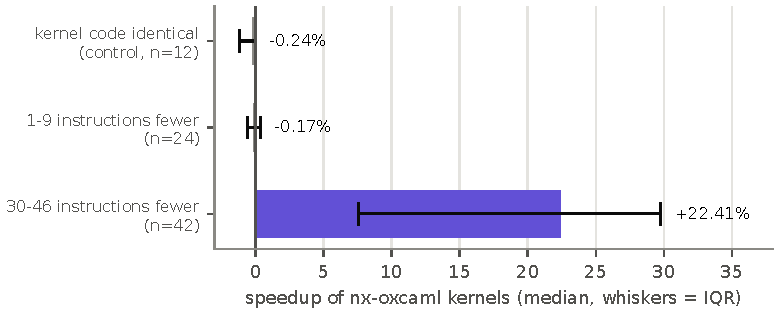
\includegraphics[width=0.66\textwidth]{fig_nx_partition}
  \caption{Speed-up from interior pointers on nx-oxcaml without safepoints (78
  cases, 21 interleaved rounds), grouped by instructions removed per kernel;
  medians with interquartile-range whiskers.}
  \label{fig:nxpart}
\end{figure}

\subsection{Bounding the Wait: Strip Mining}
Strip mining, a polled outer loop around poll-free strips of a fixed number of
iterations, keeps a fixed bound on the time to the next safepoint. Each strip
is itself a counted loop, so pointers can form inside it and are recomputed
after each outer poll; this is how HotSpot's C2 bounds the
wait~\cite{jdk_stripmining}. I did not build it. Counted loops
(Section~\ref{sec:counted}) poll at loop exits instead, with an optional trip
cap as a coarser bound; strip mining is the natural next step for bounding
latency.
